\documentclass{article}
\usepackage{spconf,amsmath,amssymb,graphicx,booktabs,array,hyperref}
\hypersetup{hidelinks}

\title{CANONICALIZING OPTION-PERMUTED VIEWS IMPROVES MATCHED-COMPUTE MULTIPLE-CHOICE INFERENCE}
\twoauthors
  {Yujie Shen}
  {School of Mathematics\\
   Hunan University, China\\
   eugeneshen2005@gmail.com}
  {Haowen Chen\sthanks{Corresponding author: Haowen Chen (hwchen@hnu.edu.cn).}}
  {College of Computer Science and Electronic Engineering\\
   Hunan University, China\\
   hwchen@hnu.edu.cn}

\begin{document}
\ninept
\maketitle

\begin{abstract}
Large language models can change their emitted answer label when the options of an otherwise identical multiple-choice question are reordered. We study Relational-Orbit inference, a parameter-free wrapper that applies the known inverse option permutation before aggregating a fixed generation budget. On the first Qwen2.5-3B public-benchmark block, mapped inference improved accuracy by 17.71 percentage points over matched-compute root inference. Two independent follow-up blocks retained a 7.29-point gain over 384 questions. On a new Mistral-7B block, the gain was 9.38 points. Shared-question panels across Qwen, Llama, Phi, Mistral and Gemma showed positive fixed-model averages, while Qwen2.5-7B ceiling effects, a negative Gemma-MMLU result, harder synthetic arithmetic and affine transformations exposed clear limits. Correct maps consistently outperformed randomized maps. The method is useful for validated four-option settings, but does not provide universal model or transformation improvements.
\end{abstract}

\begin{keywords}
multiple-choice inference, self-consistency, permutation alignment, test-time inference, language models
\end{keywords}

\section{INTRODUCTION}
Multiple-choice language-model evaluation couples a semantic decision with a surface coordinate. Reordering the answer options changes the mapping between these two objects, and models are known to be sensitive to option order and position~\cite{zheng2023selectors,pezeshkpour2024order}. Standard self-consistency aggregates sampled labels as if all samples already shared one coordinate system~\cite{wang2023selfconsistency}. Consequently, transformed prompts can create apparent disagreement even when the model selects the same semantic option.

We test a narrow correction for this mismatch. Let a canonical question have four options and let $g$ be a known cyclic option permutation. A label emitted in the transformed view is mapped through $g^{-1}$ before aggregation. We call this procedure \textsc{Relational-Orbit} (RO) inference. It uses no parameter updates and holds the total generation budget fixed against a root-only baseline. Unlike listwise permutation self-consistency~\cite{tang2024middle}, RO explicitly canonicalizes a four-way answer coordinate before pooling.

Our claim is deliberately bounded. We ask whether exact option-space alignment improves matched-compute accuracy on four-option tasks, and characterize when it fails. We report the initial public-benchmark results, disjoint follow-up blocks, shared-question cross-model panels, compute scaling, label-free selective prediction, synthetic controls and a test-time reinforcement-learning (TTRL) diagnostic. Uncertainty analyses and all raw records are archived in the project repository; the main paper emphasizes effect sizes and experimental units for readability.

Figure~\ref{fig:ro_pipeline} summarizes the complete inference path and the matched-compute controls used throughout the study.

\begin{figure*}[t]
\centering
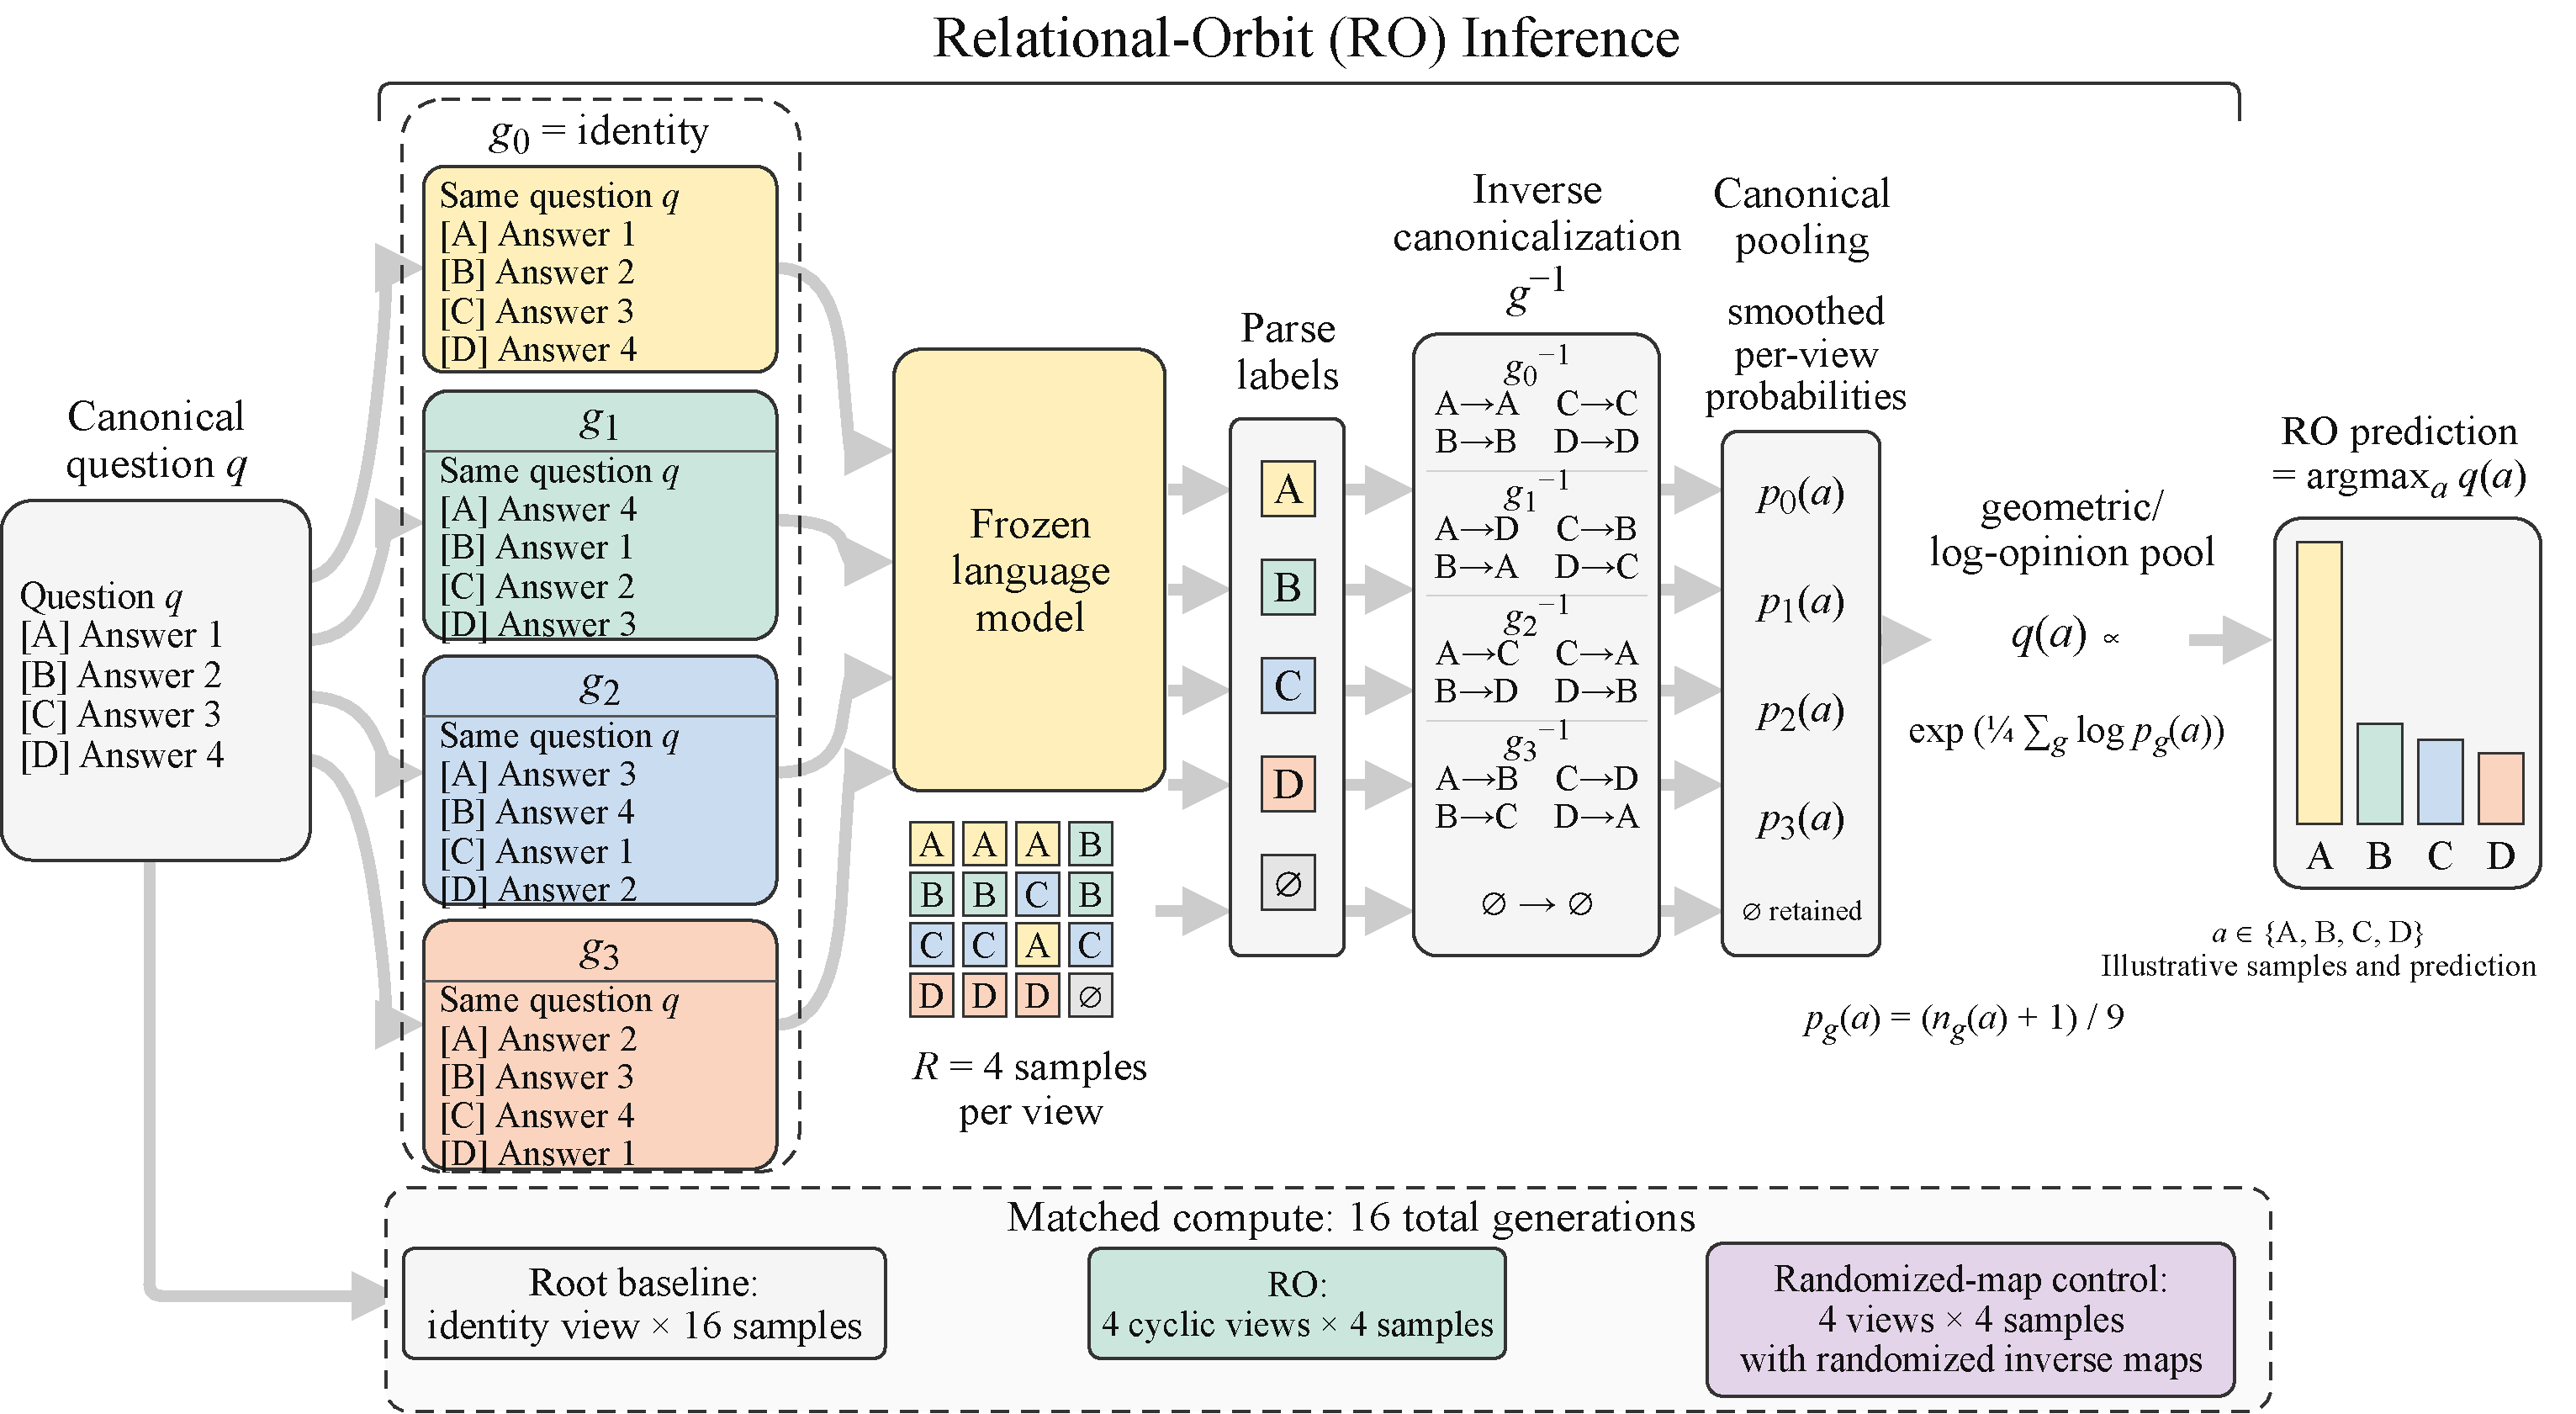
\includegraphics[width=0.96\textwidth]{figures/drawio/ro_pipeline.pdf}
\caption{Relational-Orbit inference pipeline. The canonical question is rendered in an identity view and three cyclic option permutations. A frozen language model produces four samples per view; valid labels are parsed, mapped back through the exact inverse permutation, and combined with a smoothed canonical log-opinion pool. The Root baseline spends all 16 generations on the identity view, whereas the randomized-map control preserves the same prompts and generations but destroys the known correspondence. The final prediction is the maximum of the canonical pooled distribution.}
\label{fig:ro_pipeline}
\end{figure*}

\section{RELATED WORK}
Self-consistency samples multiple reasoning paths and aggregates their final answers, extending chain-of-thought and zero-shot reasoning without parameter updates~\cite{wei2022chain,kojima2022zero,wang2023selfconsistency}. RO retains this matched-compute sampling perspective but changes the coordinate system in which samples are pooled. The distinction matters when a prompt transformation changes the surface label while preserving the semantic candidate.

Language-model decisions can exhibit label, position and recency biases~\cite{zhao2021calibrate,zheng2023selectors,pezeshkpour2024order}. Existing order-sensitivity studies motivate controlled option reorderings, but do not prescribe an inverse-map estimator for aggregating transformed labels. Permutation self-consistency addresses listwise ranking by marginalizing candidate-list orderings~\cite{tang2024middle}; our setting instead has a finite four-way label space, a known cyclic action and an exact inverse for every sample. Randomized-map and unmapped controls isolate this relational signal from the generic diversity obtained by changing prompts.

Our work is an inference-time alignment study within test-time computation~\cite{snell2025scaling}, rather than a new model architecture. The central comparison keeps prompts, checkpoints and total generations fixed, so any gain is attributable to how transformed observations are represented and pooled. This framing also makes negative results informative: a valid transformation can still hurt when model errors are coherent or when the root baseline is already near a ceiling.

\section{METHOD}
\subsection{Relational views and parsing}
For each question, the identity view and three cyclic rotations form $G=C_4$. The model produces $R=4$ sampled labels per view. A parser maps valid labels to $\{0,1,2,3\}$ and parser failures to $\varnothing$. The identity view is the root coordinate system; every transformed prompt retains the question stem and answer content and changes only the option positions. Across the four views, a fixed-position shortcut is exposed to all canonical candidates rather than being tied to one label.

\subsection{Canonical pooling and controls}
For view $g$, smoothed counts define
\begin{equation}
 p_g(a)=\frac{n_g(a)+1}{R+5},
\end{equation}
and the canonical log-opinion pool is
\begin{equation}
 q(a)\propto\exp\left(\frac{1}{|G|}\sum_{g\in G}\log p_g(a)\right).
\end{equation}
The RO prediction is $\arg\max_{a\in\{0,1,2,3\}}q(a)$. The matched-compute Root baseline uses 16 samples from the identity view and majority vote. The unmapped baseline pools transformed labels without inversion. A randomized-map control composes each non-identity inverse with an independently sampled label permutation, preserving prompts and generated text while destroying relational correspondence.

The parser-failure symbol is retained in normalization and is never silently discarded. Ties use the lowest canonical index. The primary estimand is the paired per-question contrast between Mapped and Root correctness. Because all views for one question share the same stem and reference answer, the question is the independent unit; completions are repeated observations, not independent samples. The map-control contrast is computed from 20 random inverse-map draws applied to the same stored generations.

\subsection{Adaptation and label-free reliability}
For the secondary TTRL diagnostic, leave-one-out pooled probabilities become soft rewards. Rewards are centered within each prompt and weight the full completion log-probability, with a KL penalty to the frozen reference model. We used LoRA~\cite{hu2022lora} rank 8, learning rate $10^{-5}$, $\beta=0.02$, one on-policy pass and target modules $q_{\mathrm{proj}}$ and $v_{\mathrm{proj}}$. Root TTRL receives the same sequence budget on the identity view. This diagnostic is deliberately separated from the primary inference result because policy optimization introduces additional variance.

We also compute a label-free stability score by omitting each transformed view in turn and measuring the fraction of leave-one-view-out predictions equal to the full prediction. Examples are ranked by stability, then by the pooled margin between the two largest answer probabilities, then by content hash. Accuracy at fixed coverage is consequently obtained without using ground-truth labels for selection~\cite{geifman2017selective}.

For every question, the primary effect is Mapped correctness minus Root correctness. The independent unit is the question, not a completion or a model-question pair. Shared panels reuse the same questions across fixed checkpoints; their averages therefore preserve question-level pairing. All experiments used deterministic content-hash manifests, fixed prompts and frozen checkpoints. The standard setting used temperature 0.8, top-$p$ 0.95, 192 maximum new tokens and 16 total completions per question.

\section{EXPERIMENTAL DESIGN}
\subsection{Models, data and compute}
We evaluated Qwen2.5-3B-Instruct and Qwen2.5-7B-Instruct~\cite{yang2024qwen25}, Llama-3.2-3B-Instruct~\cite{dubey2024llama}, Phi-3.5-mini-Instruct~\cite{abdin2024phi}, Mistral-7B-Instruct-v0.3~\cite{jiang2023mistral} and Gemma-2-2B-it~\cite{team2024gemma2} on eligible four-option questions from ARC-Challenge~\cite{clark2018arc}, OpenBookQA~\cite{mihaylov2018openbookqa} and MMLU~\cite{hendrycks2021mmlu}. Inference used FP16 on one RTX 3090 (24 GB), temperature 0.8, nucleus sampling with top-$p$ 0.95~\cite{holtzman2020curious}, and 192 maximum new tokens unless noted. The standard setting is four views and four completions per view, or 16 total generations per question.

The initial Qwen3B and Qwen7B blocks used 64 questions per benchmark. A first shared block used the same 192 questions for Qwen3B, Qwen7B and Llama3B; a frozen extension used those hashes for Phi, Mistral and Gemma. Later, two disjoint Qwen3B blocks, one disjoint Qwen7B block and a second shared Gemma/Phi/Mistral block were collected without tuning on evaluation questions. Dataset snapshots were mirrored locally and fingerprinted in each manifest.

\subsection{Question blocks and statistical protocol}
Question selection was deterministic using content hashes. The initial transfer, adaptation and original Llama blocks were disjoint. The shared block selected 64 questions per benchmark after removing all prior hashes. The two Qwen3B follow-ups used new offsets and were combined only after both blocks finished; the Qwen7B precision block excluded every prior 7B manifest; the later Gemma/Phi/Mistral block excluded the first family panel. Shared-model averages therefore preserve question-level pairing, whereas within-model replications pool disjoint questions.

All results below report Root accuracy, Mapped accuracy, their percentage-point difference and the correct-map advantage over randomized controls. Paired bootstrap analyses were run within benchmark strata and the same resampling indices were applied to every fixed checkpoint in a shared panel. The paper deliberately omits interval estimates from the main tables for readability; full-precision uncertainty records and gate calculations remain in the repository. No evaluation question was used for tuning or checkpoint selection.

\section{RESULTS}
\subsection{Mechanism and synthetic recovery}
The CPU simulator first isolated the intended mechanism from language-model behavior. With 10,000 simulated orbits, dispersed shortcut errors produced 1.000 Mapped accuracy versus 0.125 Root accuracy (+87.5 points). A stable shortcut produced 0.020 Mapped versus 0.125 Root, while a coherently wrong regime produced zero for both. Thus alignment can repair view-specific coordinate errors but cannot correct a shared semantic mistake.

The easy synthetic Qwen2.5-3B pilot reproduced this recovery effect: two 64-orbit blocks yielded +26.56 and +25.00 points, with correct-map advantages over randomized maps above 43 points. Truth-support coverage was at least 96.9\% and parse failure was about 2\%. A harder medium-arithmetic gate used two or three operations and moduli 11, 13, 17 or 19; its two seeds gave +12.50 and $-1.56$ points and failed the frozen gate. A post-gate easy reference reproduced a +31.25-point gain, supporting a capability boundary rather than implementation drift.

\begin{table}[t]
\centering\small\setlength{\tabcolsep}{2.2pt}
\caption{Synthetic recovery and transformation boundaries. Differences are Mapped minus Root; map control is Mapped minus randomized-map accuracy (percentage points).}
\label{tab:synthetic}
\begin{tabular}{@{}lrrrrr@{}}
\toprule
Condition & $n$ & Root & Mapped & Diff. & Map ctrl.\\
\midrule
Easy, 808 & 64 & 54.7 & 81.3 & +26.6 & +43.4\\
Easy, 909 & 64 & 57.8 & 82.8 & +25.0 & +44.3\\
Medium, 6808 & 64 & 31.3 & 43.8 & +12.5 & +12.3\\
Medium, 6909 & 64 & 32.8 & 31.3 & $-1.6$ & +7.2\\
Boolean negation & 32 & 31.3 & 37.5 & +6.3 & $-0.9$\\
Affine scale+shift & 32 & 59.4 & 53.1 & $-6.3$ & +23.6\\
Affine shift-only & 32 & 87.5 & 68.8 & $-18.8$ & +29.5\\
\bottomrule
\end{tabular}
\end{table}

Boolean negation did not exceed its randomized control. Although affine maps beat randomized gauges, they reduced accuracy relative to Root by 6.25 and 18.75 points. Exact knowledge of a transformation is therefore insufficient: the transformation must interact favorably with the model's error distribution.

\subsection{Public-benchmark transfer}
The initial Qwen3B block improved all three benchmarks and yielded a +17.71-point pooled gain. The disjoint Qwen7B confirmation yielded a smaller +5.21-point gain from a higher Root baseline. In both cases, the correct-map advantage over randomized maps was large, showing that prompt diversity alone did not explain the effect.

\begin{table}[t]
\centering\small
\caption{Initial public-benchmark transfer. Each benchmark row contains 64 questions; pooled rows contain 192 questions. Values are percentages except differences, which are percentage points.}
\label{tab:public}
\begin{tabular}{@{}llrrrr@{}}
\toprule
Model & Benchmark & Root & Mapped & Diff. & Map ctrl.\\
\midrule
3B & ARC-Challenge & 46.9 & 75.0 & +28.1 & +43.2\\
3B & OpenBookQA & 75.0 & 85.9 & +10.9 & +44.8\\
3B & MMLU & 39.1 & 53.1 & +14.1 & +18.9\\
3B & Pooled & 53.6 & 71.4 & \textbf{+17.7} & +35.6\\
\midrule
7B & Pooled & 79.7 & 84.9 & \textbf{+5.2} & +40.4\\
\bottomrule
\end{tabular}
\end{table}

\subsection{Cross-model transfer and independent replication}
On the first shared block, the Qwen/Llama fixed-model average gain was +3.13 points and the map-control advantage was +34.67 points. Model-level effects were +7.29 for Qwen3B, +2.60 for Qwen7B and $-0.52$ for Llama3B. On the same questions, the Phi/Mistral/Gemma average was +3.65 points with a +34.23-point map control. These averages are descriptive fixed-panel summaries rather than claims about a population of all models.

\begin{table}[t]
\centering\small\setlength{\tabcolsep}{2.5pt}
\caption{Matched cross-model results on the first shared 192-question block.}
\label{tab:families}
\begin{tabular}{@{}lrrrr@{}}
\toprule
Model/panel & Root & Mapped & Diff. & Map ctrl.\\
\midrule
Qwen2.5-3B & 62.0 & 69.3 & +7.3 & +31.6\\
Qwen2.5-7B & 82.3 & 84.9 & +2.6 & +40.2\\
Llama-3.2-3B & 75.0 & 74.5 & $-0.5$ & +32.2\\
Qwen/Llama avg. & 73.1 & 76.2 & +3.1 & +34.7\\
\midrule
Phi-3.5-mini & 80.2 & 82.3 & +2.1 & +36.8\\
Mistral-7B & 66.7 & 71.9 & +5.2 & +30.9\\
Gemma-2-2B & 72.4 & 76.0 & +3.6 & +34.9\\
Phi/Mistral/Gemma avg. & 73.1 & 76.7 & +3.6 & +34.2\\
\bottomrule
\end{tabular}
\end{table}

The independent blocks sharpened the main result (Table~\ref{tab:replication}). Two new Qwen3B blocks gave +6.77 and +7.81 points; pooled over 384 independent questions, Root was 59.38\% and Mapped was 66.67\%. Qwen7B remained near its ceiling after combining its original and new blocks (+0.52 points). The strongest new cross-family result was Mistral-7B: 69.27\% Root versus 78.65\% Mapped (+9.38 points). Phi improved by +2.60 points, whereas Gemma changed by $-0.52$ points overall and by $-10.94$ points on MMLU.

\begin{table}[t]
\centering\small
\caption{Independent new-sample replication at $N=16$. The final row averages three fixed models over the same 192 questions.}
\label{tab:replication}
\setlength{\tabcolsep}{2pt}
\begin{tabular}{@{}lrrrrr@{}}
\toprule
Model/panel & $n$ & Root & Mapped & Diff. & Map ctrl.\\
\midrule
Qwen3B, two blocks & 384 & 59.4 & 66.7 & \textbf{+7.3} & +30.3\\
Qwen7B, pooled & 384 & 84.4 & 84.9 & +0.5 & +39.6\\
Gemma, new & 192 & 75.5 & 75.0 & $-0.5$ & +32.6\\
Phi, new & 192 & 79.2 & 81.8 & +2.6 & +37.7\\
Mistral, new & 192 & 69.3 & 78.6 & \textbf{+9.4} & +35.8\\
Three-model avg. & 192 & 74.7 & 78.5 & +3.8 & +35.4\\
\bottomrule
\end{tabular}
\end{table}

\subsection{Budget, reliability and boundaries}
Stored generations enabled a no-new-call budget analysis. Qwen3B changed from +2.9 to +7.3 points as $N$ increased from 4 to 16, while Mistral changed from +0.5 to +9.4. Phi and Gemma were stronger at lower budgets, and Qwen7B remained close to zero. Thus the prespecified $N=16$ result is not a universally optimal budget. At 50\% label-free stability coverage, mapped accuracy ranged from 91.7\% to 96.9\% across the five independent follow-up sets.

\begin{table}[t]
\centering\small\setlength{\tabcolsep}{3pt}
\caption{Budget ablation and label-free selective accuracy on independent follow-up sets. Entries are Mapped minus Root (percentage points), except the final column.}
\label{tab:scaling}
\begin{tabular}{@{}lrrrr@{}}
\toprule
Model & $N=4$ & $N=8$ & $N=16$ & 50\% cov.\\
\midrule
Qwen2.5-3B & +2.9 & +6.3 & +7.3 & 91.7\\
Qwen2.5-7B & $-1.0$ & +0.8 & +0.5 & 96.9\\
Gemma-2-2B & +2.6 & +4.2 & $-0.5$ & 92.7\\
Phi-3.5-mini & +5.2 & +3.6 & +2.6 & 94.8\\
Mistral-7B & +0.5 & +5.2 & +9.4 & 92.7\\
\bottomrule
\end{tabular}
\end{table}

Controlled synthetic tests explain the boundary. Easy arithmetic produced +25.00 to +26.56 points across two seeds, whereas medium arithmetic gave +12.50 and $-1.56$ points. Boolean negation did not beat the randomized-map control, and affine scale-plus-shift and shift-only transformations reduced accuracy relative to Root by 6.25 and 18.75 points. In a five-seed easy synthetic TTRL study, mapped adaptation exceeded root adaptation by +5.65 points. The real-benchmark TTRL diagnostic was only +2.08 points, with benchmark effects of $-0.78$, +3.91 and +3.13 on ARC-Challenge, OpenBookQA and MMLU; it is therefore exploratory.

Hard vote and log-opinion pooling were close and neither uniformly dominated, so the full-support pool remains primary. The leave-one-view-out stability score provided a label-free ranking signal: at 50\% coverage, Mapped accuracy ranged from 91.67\% to 96.88\%. These selective results are descriptive and have not been calibrated for an unseen deployment distribution.

\section{DISCUSSION}
The evidence supports a simple interpretation: when model errors contain a coordinate-dependent component, exact inverse alignment converts transformed views into evidence about one semantic answer. The randomized-map controls are decisive for this interpretation. Prompt diversity alone was not sufficient; the known correspondence produced large advantages over random gauges across all tested families.

The effect is heterogeneous. Qwen2.5-3B retained a +7.29-point gain over 384 independent follow-up questions, and Mistral-7B supplied a separate +9.38-point result. Qwen2.5-7B changed by only +0.52 points after 384 questions, consistent with its 84.38\% Root ceiling. Gemma was neutral overall on its new block and negative on MMLU, while Llama was slightly negative on the first shared block. More samples strengthened Qwen3B and Mistral but not every model, so baseline accuracy and budget affect opportunity without fully determining the outcome.

Several limitations define the intended scope. All public tasks use four options and the transformations are cyclic. Fixed-model averages describe only the tested checkpoints; shared blocks provide paired sensitivity, whereas later blocks test transfer to new content. We do not yet provide a unified head-to-head comparison with every permutation-aware aggregator. RO should therefore be validated per task with an explicit generation budget and randomized-map control. It is a parameter-free wrapper for favorable coordinate-dependent error regimes, not a universal improvement guarantee.

\section{CONCLUSION}
RO inference makes a known option-space relation explicit before self-consistency pooling. Across initial public benchmarks, disjoint Qwen3B replication and an independent Mistral block, it produced positive matched-compute gains and consistently exceeded randomized-map controls. The strongest independent effects were +7.29 points for Qwen2.5-3B over 384 follow-up questions and +9.38 points for Mistral-7B on a separate 192-question block. These results support the narrower claim that exact alignment can improve four-option inference when model errors contain a coordinate-dependent component.

The evidence also specifies where RO should not be used. Shared panels had positive fixed-model averages but heterogeneous effects; Qwen2.5-7B was near a high Root ceiling, Llama was slightly negative on one panel, and Gemma was negative on new MMLU. More samples helped Qwen3B and Mistral but not every model. Harder arithmetic, Boolean controls and affine transformations show that a known transformation is not automatically beneficial. Mapped TTRL was positive on easy synthetic data across five seeds, whereas its real-benchmark gain was only +2.08 points and remains exploratory.

RO should be treated as a validated inference wrapper, not a universal replacement for self-consistency. Reports should state the generation budget, preserve question-level pairing, retain parser failures, include randomized-map controls and compare permutation-aware baselines. Protocols, manifests, raw records and full-precision analyses are available at \href{https://github.com/JJayshum/RO-TTRL}{github.com/JJayshum/RO-TTRL}. Future work should test larger option spaces, non-cyclic transformations and unified matched-compute baselines.

\clearpage
\section*{ACKNOWLEDGMENTS}
This work was supported by the Yuelushan Laboratory Breeding Program (grant no. YLS-2026-ZY01002), the Fundamental and Interdisciplinary Disciplines Breakthrough Plan of the Ministry of Education of China (grant no. JYB2025XDXM602), and the National Natural Science Foundation of China (grant no. 62472165).

\makeatletter
\let\rooldthebibliography\thebibliography
\renewcommand{\thebibliography}[1]{%
  \rooldthebibliography{#1}%
  \setlength{\itemsep}{0pt}%
  \setlength{\parsep}{0pt}%
}
\makeatother
\bibliographystyle{IEEEbib}
\bibliography{references}

\end{document}
